% Updated research draft, 2026-11-11; generated from the user-uploaded ACM source.
% Evidence and build provenance: leasepath_isca_v2_assets/manifest.json.
\documentclass[sigconf, screen, review]{acmart}

\settopmatter{printfolios=true}
\setcopyright{none}
\acmConference[ISCA '27]{54th IEEE/ACM International Symposium on Computer Architecture}{June 5--9, 2027}{Atlanta, Georgia, USA}
\acmYear{2027}
\acmISBN{978-x-xxxx-xxxx-x/YY/MM}
\acmDOI{XXXXXXX.XXXXXXX}
\settopmatter{printacmref=false}
\newcommand{\iscasubmissionnumber}{NaN}

\usepackage{booktabs,array,calc}
\usepackage{graphicx}
\usepackage{fancyvrb}
\usepackage{fvextra}
\usepackage{needspace}
\usepackage{xurl}
\usepackage{microtype}
\setlength{\emergencystretch}{3em}

% Longtable-compatible wrapper for full-width tables in two-column sigconf.
\newenvironment{longtable}[2][]{%
  \begin{table*}[t]\centering\small\begin{tabular}{#2}%
}{%
  \end{tabular}\end{table*}%
}
\def\endhead{}
\def\endlastfoot{}

\providecommand{\VerbBar}{|}
\providecommand{\VERB}{\Verb[commandchars=\\\{\}]}
% Keep Pandoc-generated pseudocode inside the current ACM column.
% The source contains long lines that otherwise protrude into the next column.
\DefineVerbatimEnvironment{Highlighting}{Verbatim}{commandchars=\\\{\},breaklines=true,breakanywhere=true,fontsize=\scriptsize}
\newenvironment{Shaded}{}{}
\providecommand{\AlertTok}[1]{\textcolor[rgb]{1.00,0.00,0.00}{\textbf{#1}}}
\providecommand{\AnnotationTok}[1]{\textcolor[rgb]{0.38,0.63,0.69}{\textbf{\textit{#1}}}}
\providecommand{\AttributeTok}[1]{\textcolor[rgb]{0.49,0.56,0.16}{#1}}
\providecommand{\BaseNTok}[1]{\textcolor[rgb]{0.25,0.63,0.44}{#1}}
\providecommand{\BuiltInTok}[1]{\textcolor[rgb]{0.00,0.50,0.00}{#1}}
\providecommand{\CharTok}[1]{\textcolor[rgb]{0.25,0.44,0.63}{#1}}
\providecommand{\CommentTok}[1]{\textcolor[rgb]{0.38,0.63,0.69}{\textit{#1}}}
\providecommand{\CommentVarTok}[1]{\textcolor[rgb]{0.38,0.63,0.69}{\textbf{\textit{#1}}}}
\providecommand{\ConstantTok}[1]{\textcolor[rgb]{0.53,0.00,0.00}{#1}}
\providecommand{\ControlFlowTok}[1]{\textcolor[rgb]{0.00,0.44,0.13}{\textbf{#1}}}
\providecommand{\DataTypeTok}[1]{\textcolor[rgb]{0.56,0.13,0.00}{#1}}
\providecommand{\DocumentationTok}[1]{\textcolor[rgb]{0.73,0.13,0.13}{\textit{#1}}}
\providecommand{\ErrorTok}[1]{\textcolor[rgb]{1.00,0.00,0.00}{\textbf{#1}}}
\providecommand{\ExtensionTok}[1]{#1}
\providecommand{\FloatTok}[1]{\textcolor[rgb]{0.25,0.63,0.44}{#1}}
\providecommand{\FunctionTok}[1]{\textcolor[rgb]{0.02,0.16,0.49}{#1}}
\providecommand{\BuiltInTok}[1]{\textcolor[rgb]{0.00,0.50,0.00}{\textbf{#1}}}
\providecommand{\InformationTok}[1]{\textcolor[rgb]{0.38,0.63,0.69}{\textbf{\textit{#1}}}}
\providecommand{\KeywordTok}[1]{\textcolor[rgb]{0.00,0.44,0.13}{\textbf{#1}}}
\providecommand{\NormalTok}[1]{#1}
\providecommand{\OperatorTok}[1]{\textcolor[rgb]{0.40,0.40,0.40}{#1}}
\providecommand{\OtherTok}[1]{\textcolor[rgb]{0.00,0.44,0.13}{#1}}
\providecommand{\PreprocessorTok}[1]{\textcolor[rgb]{0.74,0.48,0.00}{#1}}
\providecommand{\RegionMarkerTok}[1]{#1}
\providecommand{\SpecialCharTok}[1]{\textcolor[rgb]{0.25,0.44,0.63}{#1}}
\providecommand{\SpecialStringTok}[1]{\textcolor[rgb]{0.73,0.40,0.53}{#1}}
\providecommand{\StringTok}[1]{\textcolor[rgb]{0.25,0.44,0.63}{#1}}
\providecommand{\VariableTok}[1]{\textcolor[rgb]{0.10,0.09,0.49}{#1}}
\providecommand{\VerbatimStringTok}[1]{\textcolor[rgb]{0.25,0.44,0.63}{#1}}
\providecommand{\tightlist}{\setlength{\itemsep}{0pt}\setlength{\parskip}{0pt}}
\DefineVerbatimEnvironment{verbatim}{Verbatim}{breaklines=true,fontsize=\small}

\hypersetup{
  pdftitle={ISCA 2027 Submission},
  pdfauthor={ISCA 2027 Submission},
  pdflang={en},
  colorlinks=true,
  linkcolor=blue,
  citecolor=blue,
  urlcolor=blue,
  pdfcreator={LaTeX via acmart}}

\begin{document}

\title{LeasePath: Distribution-Aware KV Cache Retention for Tool-Augmented LLM Agents}
\author{ISCA 2027 Submission \textbf{\#\iscasubmissionnumber} -- Confidential Draft -- Do NOT Distribute!!}
\renewcommand{\shortauthors}{ISCA 2027 Submission \#\iscasubmissionnumber}

\begin{abstract}
Tool-augmented large language model agents repeatedly return to growing
conversation prefixes after uncertain tool, client, and queue delays.
LeasePath predicts the time to the next legal key--value (KV) prefix
demand and maps its finite-horizon probability mass to a discounted
retention score. A pressure-triggered controller applies the score to
legal prefix leaves, protecting active references and accounting for
shared physical occupancy. We implement native CUDA KV eviction and
audit consumed tool feedback, actual prefill, and validated deliveries.
An initial three-task experiment supports equal-cost scoring over a
calibrated cost extension. In a subsequent continuous-agent development
comparison, six authored projects execute eight user turns each with
nine tool types and identical per-project prompt sequences across five
policies. Dynamic GBDT distribution scoring reuses 329,344 additional
tokens, reduces aggregate prefill time by 44.86\%, and reduces mean
user-turn response time by 19.76\% relative to retired-first LRU, with
48/48 accepted turns in each arm. Its two online updates use only
observed event prefixes. Static GBDT and fixed-window probability
scoring achieve similar response times; this single ordered cycle on a
shared server does not establish an advantage for dynamic updates or
for distribution scoring over that window. Independent projects,
balanced repetitions, drift, and complete-system baselines remain open.

\end{abstract}
\maketitle

\section{Introduction}\label{introduction}

An LLM agent often pauses model execution to run a tool, inspect its
result, and continue generation with an extended conversation. The KV
state of the preceding context can save substantial prefill work when
that conversation resumes. During the pause, however, the state occupies
capacity that other sessions could use. Retaining every idle prefix is
infeasible under pressure, while immediately discarding it can turn a
later continuation into redundant computation. The useful question is
therefore whether an idle prefix will be needed again, when that demand
will occur, and which physically feasible retention choice is worth its
capacity. Figure~\ref{fig:agent-loop} summarizes this setting: one task
repeatedly alternates between model calls and tools, while the time to the
next legal prefix demand is estimated during each idle interval.

\begin{figure*}[t]
\centering
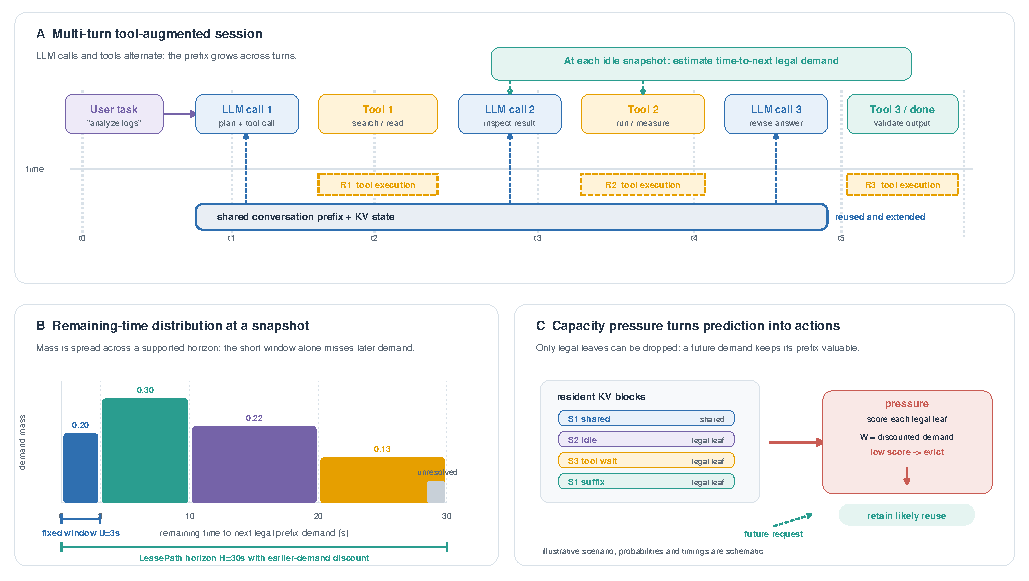
\includegraphics[width=\textwidth,keepaspectratio,alt={Schematic of a multi-turn tool-augmented session. Model calls repeatedly reuse and extend a shared KV prefix; tool execution creates waiting intervals whose remaining-time distribution is estimated and then used to choose legal retention actions under capacity pressure.}]{leasepath_isca_v2_assets/figures/figure1_agent_loop.pdf}
\caption{Workload scenario motivating LeasePath. A tool-augmented agent
reuses and extends a shared conversation prefix across multiple model
calls. At each idle snapshot, tool execution creates a distribution over
the remaining time to the next legal prefix demand; under capacity
pressure, this distribution is mapped to feasible retain/evict actions.
The timings and probability masses are schematic.}
\Description{A growing conversation alternates model calls and real tool execution. A predicted remaining-time distribution guides legal KV retention under pressure.}
\label{fig:agent-loop}
\end{figure*}

Recency captures when a prefix was last used, but it does not directly
describe progress through external computation. A tool that has been
running for several seconds may be close to completion or may still have
a long remaining duration. Workflow step distance also need not
correspond to elapsed time: one step can be a short lookup or a long
numerical computation. Even when the next-use time can be estimated, a
single scalar need not preserve all information relevant to retention.
Two prefixes can have the same probability of demand within a short
window yet assign the remaining demand probability to very different
times.

Prior work already uses tool durations, elapsed-time conditioning,
empirical distributions, workflow structure, and termination
probabilities to manage agent KV caches. In particular, CacheWise
estimates remaining tool time, Continuum selects time-to-live values
from distributions, and PBKV uses discounted probabilistic lookahead
over future invocations. LeasePath does not claim these ideas
individually. We investigate a more specific connection: a distribution
over \textbf{wall-clock time to the next legal prefix demand}, evaluated
at a causal decision snapshot, can be mapped to a retention score and
applied to the currently feasible physical eviction actions. The
resulting hypothesis is testable with a fixed predictor: preserving
timing information across a common horizon may change which useful
prefixes survive compared with evaluating the same distribution at one
time threshold.

Three issues make that hypothesis nontrivial. First, the prediction
target must correspond to demand. Tool completion, request readiness,
and cache lookup are separate events. A lookup that misses still
establishes demand, while an observation window ending does not
establish that reuse will never occur. Second, scores act on a
constrained cache. Active references cannot be evicted, a retained
descendant requires its prefix, and several owners can share one
physical block. Third, avoided prefill is only one component of
completion time. Tool variation, queueing, generation differences, and
controller overhead can offset a cache improvement.

LeasePath addresses these issues through a demand-based event
definition, a finite-horizon discounted score, and a controller that
repeatedly chooses legal leaves of the resident prefix structure. The
score integrates unconditional demand probability mass; it neither
conditions on eventual reuse nor reallocates unresolved tail mass into
the supported window. The main configuration gives all candidates the
same recomputation-cost multiplier, allowing the
distribution-to-decision mapping to be examined separately from an
estimated cost model.

The present evidence comprises a completed prototype and two development
experiments, reported separately. A three-task comparison holds the
predictor fixed to examine the scoring functional and a cost extension.
A subsequent continuous-agent comparison uses six growing project
histories, real tool feedback, and repeated user turns. Relative to
retired-first LRU, its four prediction policies reduce observed mean
user-turn response by 17.95\%--19.80\%. However, the differences among
static GBDT, dynamic GBDT, and fixed-window scoring are small; the
preferred predictor and update regime remain empirical choices. A
mixture is a candidate for future validation, not a tested result.

This draft makes three contributions within that scope:

\begin{enumerate}
\def\labelenumi{\arabic{enumi}.}
\tightlist
\item
  A prediction and measurement formulation that separates the first
  legal KV demand, explicit retirement of an owner--context
  relationship, and observation censoring, while keeping physical hit
  outcomes out of demand labels.
\item
  An implemented mapping from finite-horizon demand distributions to
  legal, pressure-triggered KV eviction, with explicit treatment of
  prefix dependencies, shared ownership, support failure, and
  deterministic tie-breaking.
\item
  An audited preliminary evaluation that measures actual prefill and
  validated-answer completion time, alongside a continuous-agent
  comparison with causally audited online updates and a negative result
  for the cost extension on the earlier workload.
\end{enumerate}

These contributions establish an implementation and an initial empirical
case. They do not establish superiority to CacheWise or Continuum, broad
generalization, or optimal cache control.

\section{Background and Related
Work}\label{background-and-related-work}

\subsection{Agent execution and prefix
reuse}\label{agent-execution-and-prefix-reuse}

During prefill, a transformer constructs KV state for input tokens;
during decoding, it extends the state as it generates output. A
compatible cached token prefix can reduce the input portion that must be
processed again. Compatibility depends on the actual tokens and the
model, tokenizer, position treatment, and KV configuration. Similar text
or a shared task identifier is insufficient.

When a model call finishes, its context may become idle while an
external tool runs. A subsequent request typically appends tool feedback
and protocol text. The tool can finish before the client constructs this
request, and a ready request can wait before the backend performs its
lookup. For a simple serial dependency, the remaining time to lookup can
be decomposed as

\[
R_{\mathrm{lookup}}=R_{\mathrm{tool}}+D_{\mathrm{client}}
 +W_{\mathrm{queue}}+D_{\mathrm{dispatch\to lookup}}.
\]

For parallel tools or branches, dependency completion replaces the
single-tool term. This decomposition explains why tool duration is an
imperfect label for cache demand; it does not imply that all components
are observable to the current predictor. The earlier frozen predictor has no
measured queue-state feature; the continuous-agent predictor adds
causally observed queue and execution state.

Our prototype runs concurrent agent sessions and tools, while serving
model requests serially in first-come, first-served (FCFS) order.
Changing retention can change service time, subsequent tool launches,
and later arrivals. Consequently, replaying a fixed baseline lookup
timeline is useful for diagnosing decisions but cannot reproduce another
policy's natural completion time.

\subsection{Time-aware KV
management}\label{time-aware-kv-management}

InferCept estimates interception duration to choose among preservation,
recomputation, and swapping (Abhyankar et al., 2024). Continuum uses
empirical tool-duration distributions to choose KV time-to-live values,
incorporating prefill or reload costs and queueing effects, and combines
retention with program-level scheduling (Li et al., 2025, version 7).
CacheWise clusters tool arguments using TF-IDF and KMeans, conditions
historical duration distributions on elapsed waiting time, and ranks
candidates using estimated next-use time (Tiwari et al., 2026).

These systems establish direct precedents for using distributions, tool
metadata, and elapsed time. Our controlled question concerns the
decision functional applied to a common prediction: a fixed-window
demand probability versus discounted mass across a finite horizon, under
the same prefix constraints. The fixed-window baseline in this draft is
\(F_U(3\,\mathrm{s})\). It is a cumulative probability, not a point
estimate of return time and not an implementation of CacheWise.
Complete-system comparisons must additionally account for scheduling,
prediction features, and available storage tiers.

\subsection{Workflow structure, lifecycle, and
sharing}\label{workflow-structure-lifecycle-and-sharing}

KVFlow uses an Agent Step Graph and steps-to-execution to prioritize
shared prefix nodes (Pan et al., 2025). Its dependencies include both
all-predecessor and alternative-predecessor conditions, and its full
system includes prefetching and scheduling. PBKV predicts future agent
invocations from workflow history, graph structure, and prefill
representations (Zheng et al., 2026). Its multistep score already
combines termination probabilities, survival across steps, confidence
discounting, and aggregation across workflows. LeasePath therefore does
not present probabilistic lookahead, termination-aware scoring, or
discounting as new in themselves. Its target is a first compatible
demand in wall-clock time, and its implementation evaluates that target
through legal prefix eviction.

Lifecycle information is also an important baseline. KVTether maps
message lifecycle information to KV states, reclaims dead state first,
and applies MRU among live-but-idle entries to exploit delayed reuse (Fu
et al., 2026). PBKV likewise prioritizes entries whose associated
workflows have terminated. Any claimed gain from distribution
information must be separated from reclaiming already retired state. We
therefore use retired-first LRU as an internal comparator; this does not
reproduce the full KVTether policy.

\subsection{Learned prediction and competing
risks}\label{learned-prediction-and-competing-risks}

Prediction-guided caching has a broader history, including Learning
Relaxed Belady for content distribution networks (Song et al., 2020).
Competing-risk time-to-event modeling is also established; DeepHit
learns time distributions for multiple competing outcomes (Lee et al.,
2018). LeasePath uses standard discrete-time competing-risk semantics,
instantiated with empirical estimators and a shared boosted-tree hazard
model. The intended contribution is the link between demand semantics,
feasible KV actions, and measured execution benefit. Neither a
tree-based predictor nor competing-risk modeling alone constitutes that
contribution. The LRB bibliographic entry still requires an independent
source recheck.

\section{Problem Formulation}\label{problem-formulation}

\subsection{The next legal demand}\label{the-next-legal-demand}

A prediction object is an idle relationship between an owner--context
version and a compatible token prefix. At decision time \(t\), its
causal history is \(\mathcal H_t\). The first subsequent outcome is
represented by \((R,J)\), where \(R>0\) is the remaining time and
\(J\in\{U,D\}\) is the event type. A relationship can also remain
unresolved throughout the observation window.

\textbf{Demand (\(U\)).} The first compatible backend lookup whose
request begins with the relationship's prefix. Both a physical hit and a
physical miss establish demand. Evicting the cached state therefore does
not turn a future positive label into a negative one.

\textbf{Retirement (\(D\)).} An explicit event terminating this
owner--context relationship. Tool completion, cache eviction, or
retirement of another owner is insufficient. A shared physical block can
remain useful to its other owners after one relationship ends.

\textbf{Censoring (\(C\)).} Observation ends while the relationship
remains open and before an observed \(U\) or \(D\). Censoring limits
what is known about the future; it is not a third competing event.
Missing logs likewise cannot be converted into retirement.

If events share a timestamp, recorded event order determines the first
outcome, including its ordering relative to observation end. Conditioned
on the relationship being open at \(t\), define the cumulative incidence
functions

\[
F_j(r\mid\mathcal H_t)=\Pr(R\le r,J=j\mid\mathcal H_t),
\qquad j\in\{U,D\},
\] \[
S(r\mid\mathcal H_t)=1-F_U(r\mid\mathcal H_t)-F_D(r\mid\mathcal H_t).
\]

Unlike a return-time distribution conditioned on eventual reuse, \(F_U\)
can have total mass below one. This distinction matters: a prefix with a
small chance of an early demand need not be preferable to one with a
large chance of a somewhat later demand. The current dataset contains no
natural censoring, so correct censoring semantics are an implementation
property rather than an empirically established robustness result.

\subsection{Feasible retention and physical
occupancy}\label{feasible-retention-and-physical-occupancy}

Let \(b\) denote a resident prefix block, \(B_b\) its payload bytes, and
\(\mathcal O_b\) its current live owner bindings. Shared blocks count
once toward physical occupancy. Feasible eviction must preserve active
references, the currently admitted request's required prefix, prefix
continuity, and consistent shared references. In the resident prefix
structure, removing an unprotected leaf preserves ancestor availability
for all remaining descendants. Removing an internal block while
retaining its dependent descendants would not.

The candidate set changes after each logical removal. A parent can
become a leaf, and the continuously reachable prefix of an owner can
shorten. A single initial ranking is therefore insufficient to describe
the implemented procedure. A request that is ready but not currently
being admitted does not acquire additional hard protection merely from
being ready.

\subsection{Evaluation objective}\label{evaluation-objective}

The external objective is shorter validated-answer completion time under
fixed resource and quality constraints. For the earlier three-task experiment,
the measured endpoint is precisely

\[
\mathrm{JCT}_i=t_i^{\mathrm{validated\ answer}}-t_i^{\mathrm{submission}}.
\]

All three tasks in a batch share a submission timestamp taken before
per-task preparation. Thus the endpoint includes preparation, queueing,
model execution, tools, controller work, and final validation. Model
loading, residency preparation, pre-batch cache clearing, and
post-validation retirement and archival work are outside this window.
This submission timestamp is distinct from each model request's cache
admission time. For continuous projects, the endpoint is instead
user-turn response: actual arrival of the current user message to an
independently validated delivery. It includes queueing, model service,
tools, controller work, and validation, and excludes user think time
before that arrival. Project makespan includes the think intervals.
These endpoints are not pooled across experiments.

LeasePath does not directly optimize expected JCT over future arrivals,
tool branches, and outputs. It uses a computable retention proxy and
measures whether the resulting actions improve the external endpoint. No
global optimality or approximation guarantee for JCT is assumed.

\section{LeasePath}\label{leasepath}

\subsection{Predicting remaining-time
distributions}\label{predicting-remaining-time-distributions}

Choose interval boundaries \(0=r_0<r_1<\cdots<r_K\). For a fixed
snapshot, the predictor produces interval-conditional probabilities
\(h_k^U,h_k^D,h_k^0\) summing to one. Here \(h_k^0\) denotes survival
through the interval, not censoring. The unconditional masses follow the
standard recursion

\[
\begin{aligned}
S_0&=1,& p_k^U&=S_{k-1}h_k^U,\\
p_k^D&=S_{k-1}h_k^D,& S_k&=S_{k-1}h_k^0.
\end{aligned}
\] \[
F_U(r_k)=\sum_{q=1}^{k}p_q^U,\qquad
F_D(r_k)=\sum_{q=1}^{k}p_q^D.
\]

Using \(h_k^U\) directly as unconditional mass would overcount outcomes
after an earlier event. Because the model already predicts remaining
time from the current snapshot, its output is not conditioned a second
time by subtracting elapsed time.

We implement global and conditional empirical estimates and a shared
LightGBM multiclass hazard model. Conditional empirical estimation
groups tool, phase, and elapsed-time bucket, with shrinkage or fallback
for small groups. The boosted-tree model receives the same information
plus interval index. Task identity, future tool output, future remaining
duration, the next request's actual length, and future cache outcomes
are excluded. Prefix identity and length are used by cache management
and validation; they are not learned features in the earlier frozen
model. The continuous-agent version retains tool identity and adds
causal execution state and current prefix length, as detailed below.

For training, completely observed survival intervals receive the waiting
label, and the event interval receives \(U\) or \(D\). A censored
partial interval and unobserved later intervals are excluded. With
snapshot weights \(a_n\) and interval masks \(m_{nk}\), the model uses a
weighted multiclass loss of the form

\[
\mathcal L=-\sum_{n,k}a_n m_{nk}\log h_k^{y_{nk}}(x_n).
\]

Snapshots from the same parent task remain in one split. Snapshot
in the earlier predictor sum to one per parent, with equal episode
weights within a parent and equal snapshot weights within an episode.
The continuous-agent version preserves these relative weights but
normalizes their mean to one; this changes their absolute scale relative
to the fixed regularization constants. Each observed risk
row inherits its snapshot weight; the loss is not additionally
normalized by the number of observed intervals. This prevents a parent
from dominating merely through snapshot count, while allowing its
observed risk duration to affect its total contribution to the interval
loss. It does not make snapshots independent or correct informative
censoring.

\subsection{A finite-horizon retention
score}\label{a-finite-horizon-retention-score}

For a common supported horizon \(H=r_m\) and discount scale \(\tau>0\),
define

\[
W_i=\sum_{k=1}^{m}\exp(-r_k/\tau)
\left[F_{U,i}(r_k)-F_{U,i}(r_{k-1})\right].
\]

The frozen configuration uses \(H=30\) seconds and \(\tau=10\) seconds.
The exponential is a deterministic preference for earlier demand, not an
estimated probability that the cache will survive. Unresolved mass after
\(H\) remains unresolved; the in-window mass is not renormalized to
imply certain reuse. Retirement already competes with demand through the
hazard recursion, so multiplying the score again by \(1-F_D\) would
count that effect twice.

The equal-cost block score is

\[
V_b=\frac{\max_{i\in\mathcal O_b}W_i}{B_b}.
\]

Low-scoring legal leaves are preferred for eviction, after unbound
leaves have been considered. Equal cost means that all
recomputation-cost multipliers are set to one; it does not assert equal
real prefill cost. All blocks in the current experiment have the same
size, so the byte denominator does not change their order. The maximum
over owners is an aggregation heuristic inherited by the implementation.
It is neither the exact probability that any owner will demand the block
nor the expected value of multiple future uses.

\textbf{Why more than one window can matter.} Consider a constructed
example with demand masses at 1, 10, and 30 seconds. Prefix A has masses
\((0.2,0.6,0)\), while B has \((0.2,0,0.6)\); the remaining 0.2 is left
unresolved. Both have \(F_U(3\,\mathrm{s})=0.2\). With \(\tau=10\)
seconds, however,

\[
\begin{aligned}
W_A&=0.2e^{-0.1}+0.6e^{-1}\approx0.402,\\
W_B&=0.2e^{-0.1}+0.6e^{-3}\approx0.211.
\end{aligned}
\]

The fixed-window score cannot distinguish them, whereas the discounted
score prefers retaining A under equal costs and feasibility. This
illustrates an information difference, not a measured benefit or a claim
that A always yields lower JCT.

\begin{figure*}[t]
\centering
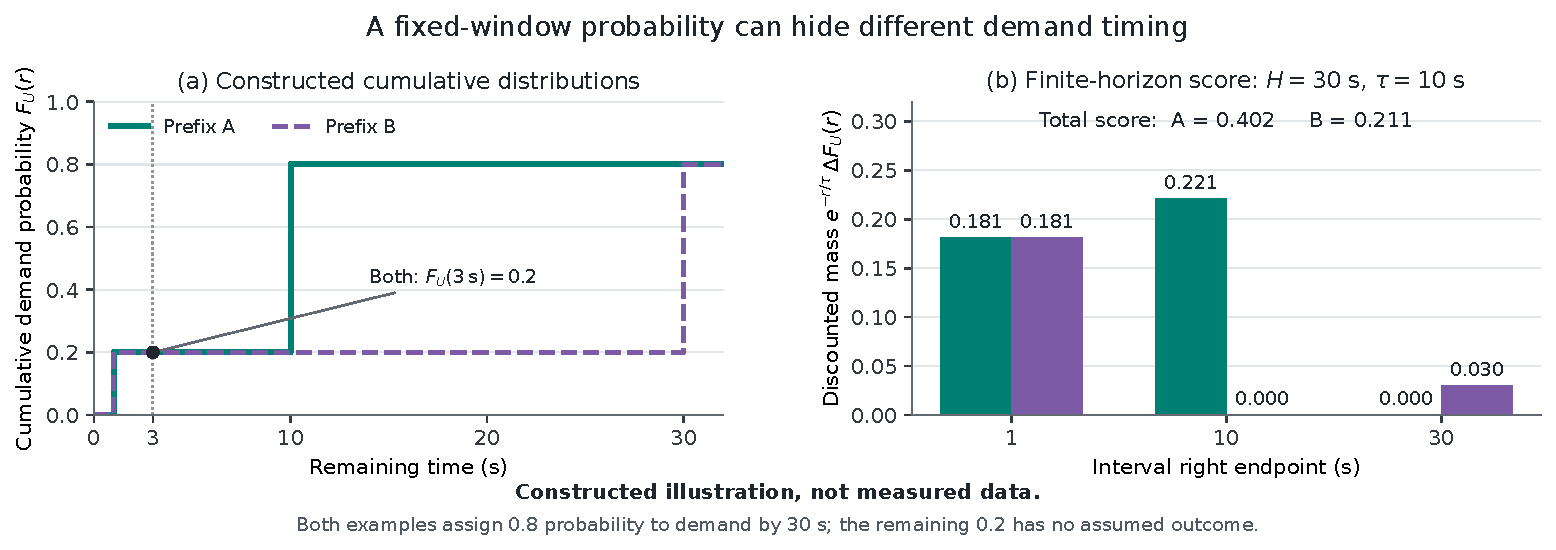
\includegraphics[width=\textwidth,keepaspectratio,alt={Constructed illustration, not measured data. A and B have equal three-second cumulative demand probability and equal demand mass through 30 seconds, but different temporal allocations and discounted scores. Unresolved mass is not reassigned to demand.}]{leasepath_isca_v2_assets/figures/figure1_distribution_example.pdf}
\caption{Constructed illustration, not measured data. A and B have equal
three-second cumulative demand probability and equal demand mass through
30 seconds, but different temporal allocations and discounted scores.
Unresolved mass is not reassigned to
demand.}\Description{Two illustrative demand distributions share the same three-second cumulative probability but have different discounted mass through thirty seconds.}
\label{fig:distribution-example}
\end{figure*}

The score has simple interpretive properties. Right-endpoint discounting
lower-bounds the corresponding continuous discounted functional of the
same distribution; pointwise dominance of cumulative demand
probabilities on the grid preserves the discrete score ordering.
The finite-grid analysis gives these facts and a conditional perturbation bound. They
explain the proxy and do not establish optimal cache decisions.

\subsection{Pressure-triggered legal
eviction}\label{pressure-triggered-legal-eviction}

Algorithm 1 describes the main equal-cost policy. The controller fixes
one decision time for an admission and memoizes each encountered owner's
prediction. It removes one logical leaf at a time, recomputing feasible
leaves and live bindings. The completed deletion plan is then submitted
to the native backend; the implementation does not invoke a separate
native deletion after every logical comparison.

\Needspace{30\baselineskip}

\textbf{Algorithm 1: LeasePath admission and eviction.}

\begin{Shaded}
\begin{Highlighting}[]
\NormalTok{Input: compatible request prefix, resident tree, references,}
\NormalTok{       frozen predictor, admission timestamp t0}
\NormalTok{1. Validate ancestry, request size, and protected{-}capacity feasibility.}
\NormalTok{2. Protect active blocks and the current request\textquotesingle{}s prefix.}
\NormalTok{3. Initialize an owner memo using fixed t0, and an empty drop plan.}
\NormalTok{4. fallback \textless{}{-} false}
\NormalTok{5. While the request cannot fit within the persistent quota:}
\NormalTok{     Recompute unprotected leaves and reachable owner bindings.}
\NormalTok{     If unbound leaves exist:}
\NormalTok{         Choose one by (touched, {-}depth, key).}
\NormalTok{     Otherwise:}
\NormalTok{         Predict newly encountered owners once, using state at t0.}
\NormalTok{         If any required distribution score is unavailable:}
\NormalTok{             fallback \textless{}{-} true}
\NormalTok{         If fallback:}
\NormalTok{             Choose a leaf by the retired{-}first LRU ordering.}
\NormalTok{         Otherwise:}
\NormalTok{             Choose the minimum (V\_b, touched, {-}depth, key).}
\NormalTok{     Remove the leaf from the logical tree; append to drop plan.}
\NormalTok{6. Submit the drop plan to native KV storage; verify mappings/cells.}
\NormalTok{7. Call native generation, which checks native request bounds.}
\NormalTok{8. On normal model completion, release its context to idle.}
\NormalTok{   On abort, clean up unmaterialized suffix and active ownership.}
\end{Highlighting}
\end{Shaded}

Admission fails when protected active state makes the request
infeasible; the controller does not violate active-reference constraints
to force progress. The fixed timestamp is passed to the logical
controller at admission. Native generation bounds are checked when
generation is invoked, after the deletion plan has been applied; the
prototype does not guarantee that every backend rejection precedes all
cache changes. A missing or invalid distribution triggers LRU ordering
for the remainder of that admission. Previously selected actions are not
retroactively undone. Without capacity pressure, scoring is unnecessary.

The current implementation scans candidates and updates the logical
structure repeatedly. Its prediction memo reduces repeated calls within
an admission, but it does not provide a heap-based logarithmic eviction
algorithm. Scalability depends on the number of owners, candidate
leaves, and required removals, and needs measurement beyond the present
small setting.

\subsection{Support and fallback}\label{support-and-fallback}

The distribution score requires the horizon to coincide with an
available right endpoint and every interval through \(H\) to have at
least five training workflows in its global risk support. At the
30-second interval, both the earlier frozen training data and the
initial continuous-agent data provide only six workflows.
Passing the support gate therefore does not imply a reliable statistical
confidence bound.

Unseen tool, phase, or elapsed categories invoke the predictor's
training-global fallback in the earlier predictor. The continuous-agent
GBDT instead maps unseen tools to an unknown category and retains the
state features; deterministic training-only masking of approximately
one tenth of episodes trains that category. An unsupported compatibility
class yields an unsupported distribution. These are different from the controller
falling back to LRU because the common window is unavailable. Invalid
probability output is recorded as an error, not silently interpreted as
zero demand or retirement.

The fixed-window comparator checks support at its three-second output.
Its implementation does not impose the distribution policy's additional
five-workflow condition across the whole 30-second horizon. These
support rules must not be described as identical. No distribution
fallback was observed in the earlier natural experiment, but
comparisons under support failure require separate analysis.

\subsection{Cost-weighted extension}\label{cost-weighted-extension}

We also implement a cost multiplier using an independently calibrated
prefill table. Let \(P_i\) be the currently observed, block-aligned
prefix length and \(\ell_i\) the continuously resident prefix length.
For 128-token blocks, the estimated marginal cost is

\[
\begin{aligned}
\widehat C_{i,b}&=\widehat T(P_i+1,\ell_i-128)\\
 &\quad-\widehat T(P_i+1,\ell_i),\\
V_b^{\mathrm{cost}}&=\frac{\max_{i\in\mathcal O_b}
 (\widehat C_{i,b}W_i)}{B_b}.
\end{aligned}
\]

The extra token satisfies the backend's requirement to leave an uncached
token in the calibration request; it is not a prediction of the future
suffix. The table uses exact supported grid points without interpolation
or extrapolation. Missing cost support switches the remaining admission
comparisons to equal cost, separately from distribution-to-LRU fallback.
Continuous resident length and marginal cost are updated after logical
removals.

This extension is an ablation, not part of the main successful
configuration. It underperforms equal-cost scoring in the current
experiment. A good fit on calibration prompts does not by itself
establish a good estimate of the cost of a future request containing new
tool output.

\subsection{Native realization}\label{native-realization}

The adapter executes real KV reference deletion and checks physical
token/cell mappings around requests. Shared payload is counted once, and
generated outputs and consumed tool feedback are linked to the event
stream. The backend preallocates its device KV buffer. Eviction frees
used cells and references for reuse within that allocation; it does not
shrink reserved CUDA memory. We distinguish the persistent payload
quota, used physical cells, and reserved device bytes. The logical
blocks should not be equated with the implementation of paged blocks in
another serving engine.

\section{Experimental Design}\label{experimental-design}

\subsection{Questions and evidence
units}\label{questions-and-evidence-units}

The earlier experiments address whether a different functional of the
same predictor changes actual reuse and measured completion time,
whether the frozen predictor improves on empirical estimates, and
whether a marginal-cost multiplier helps. The continuous-agent
comparison additionally examines real multi-turn reuse and deployable
online updates; its single cycle is not an isolated adaptation test. Independent-task
generalization, comparison with complete prior systems, broad cache
pressure, and full overhead amortization remain open.

Table 1 separates the earlier data used for these questions. A parent task is
the grouping unit for prediction evaluation. The online experiment
repeats three known parents in four time cycles; it does not contain 48
independent task types.

\begin{table*}[t]
\centering\small
\begin{tabular}{@{}
  >{\raggedright\arraybackslash}p{(\linewidth - 6\tabcolsep) * \real{0.2500}}
  >{\raggedleft\arraybackslash}p{(\linewidth - 6\tabcolsep) * \real{0.2500}}
  >{\raggedright\arraybackslash}p{(\linewidth - 6\tabcolsep) * \real{0.2500}}
  >{\raggedright\arraybackslash}p{(\linewidth - 6\tabcolsep) * \real{0.2500}}@{}}
\toprule\noalign{}
\begin{minipage}[b]{\linewidth}\raggedright
Evidence set
\end{minipage} & \begin{minipage}[b]{\linewidth}\raggedleft
Parent tasks
\end{minipage} & \begin{minipage}[b]{\linewidth}\raggedright
Episodes / snapshots
\end{minipage} & \begin{minipage}[b]{\linewidth}\raggedright
Role
\end{minipage} \\
\midrule\noalign{}
\endhead
\bottomrule\noalign{}
\endlastfoot
Current-server development collection & 50 & 150 / 347 & Data and
predictor development \\
Internal training subset & 40 & 119 / 275 & Frozen estimators \\
Internal evaluation subset & 10 & 31 / 72 & Same-source prediction
evaluation \\
Natural policy experiment & 3 known parents & 48 task executions, 16
batches & Four-policy comparison \\
\end{tabular}
\caption{Completed evidence only. The 50-task collection has episode outcomes \(U/D/C=100/50/0\); train and evaluation subsets have \(79/40/0\) and \(21/10/0\), respectively. Online task executions and prediction episodes are different units.}
\end{table*}


The development tasks are local data-analysis workloads spanning SQL,
machine learning, cleaning, statistics, time series, and numerical
analysis. They share authorship, libraries, and some data structures.
The collection initially succeeded on 49 of 50 parents; after retaining
the failed attempt and rerunning the complete 38-task extension batch,
the accepted collection contains 50 successful parents. The prediction
results therefore describe the accepted collection, not a 100\%
first-attempt success rate. Historical data from a different server and
earlier Codex/MBPP workflows are not merged into these counts.

\subsection{Prediction protocol}\label{prediction-protocol}

The 40/10 split was fixed by semantic strata and a hash-based ordering
with seed 23 before fitting. Entire parents, their episodes, and
snapshots remain together. All 50 tasks had already been inspected
during development, so the split is an internal holdout, not an
untouched final test. The estimators use training-only vocabularies and
support counts, with no parameter search, early stopping, or refit on
all 50 parents.

We report the parent-weighted cumulative three-class Brier score for
\((F_U,F_D,S)\); its range is 0--2, and lower is better. It is not
answer accuracy. The same snapshots and supported windows are used
across predictors. The predictor settings are summarized in this section.
The test snapshots contain no demand within 0.1 seconds, even though
that horizon was the original primary prediction metric. Longer,
decision-relevant horizons are therefore reported alongside it.

\subsection{Execution platform and controlled
comparisons}\label{execution-platform-and-controlled-comparisons}

The native backend serves Qwen2.5-Coder-32B-Instruct from an unquantized
F16 GGUF model with F16 KV storage, using llama.cpp/CUDA and three V100
GPUs with 32 GiB each. The model is split by layers across GPUs. The
physical context is 16,384 tokens. Each managed block holds 128 tokens
and represents 32 MiB of KV payload. The earlier experiment uses 24
persistent blocks, equivalent to 3,072 tokens or 768 MiB of payload, and
2,048 tokens of transient headroom. Model requests run serially in FCFS
order; three sessions and their tools can overlap. Each tool uses one
numerical thread.

The four policies share inputs, model, execution protocol, native
controller, legal action space, unbound-state reclamation, tie-breaking,
resource settings, and auditing:

\begin{itemize}
\tightlist
\item
  \textbf{A, retired-first LRU:} reclaim unbound legal leaves first,
  then order live candidates by recency.
\item
  \textbf{B, fixed-window probability:} use \(F_U(3\,\mathrm{s})\) from
  the frozen GBDT, with equal costs.
\item
  \textbf{C, LeasePath equal cost:} use the same GBDT and \(W\) with
  \(H=30\) seconds and \(\tau=10\) seconds.
\item
  \textbf{D, LeasePath with cost:} multiply the same discounted mass by
  calibrated marginal cost.
\end{itemize}

The code identifier \nolinkurl{gbdt_point} refers to B, but we use
``fixed-window probability'' throughout the paper to avoid confusing it
with a time prediction. Conditional empirical prediction has been
evaluated offline; its online combination with the same distribution
controller is measured in the subsequent continuous-agent experiment.

The online parents are logistic holdout evaluation, ridge
cross-validation, and temporal as-of matching. All three belong to the
previously viewed ten-parent internal evaluation subset. Each policy
executes one three-session batch in each of four cycles, using a
Williams order: A--B--D--C, B--C--A--D, C--D--B--A, and D--A--C--B.
Every policy occupies each position once, and each directed adjacent
pair appears once. This balances order in this small experiment; it does
not create additional independent workloads.

\subsection{Measurement, quality, and
interference}\label{measurement-quality-and-interference}

JCT is measured from common batch submission to independently validated
final answers as defined in Section 3.3. Cached tokens, actual prefill
tokens, prefill time, and controller measurements are aggregated per
three-session batch. JCT is averaged per task. Overlapping tool times
and aggregate model times cannot simply be added to reconstruct a task's
critical path.

All policies run real tools and consume their results in subsequent
actual prompts. Final acceptance checks the response schema, output
artifacts, task references, and feedback consumption. The completed
experiment contains 144 live generations and 13 native probes; a
separate traced diagnostic is excluded from natural timing. We report
all 48 task executions in the completed comparison, all of which pass
validation.

The server is shared. Fixed CPU affinity, numerical thread limits,
NUMA/THP controls, pinned model and dependency pages, and prospective
I/O and major-fault gates reduce specific interference sources. They do
not reserve CPU cores or memory bandwidth. A violation stops the attempt
and remains in the evidence; slow observations are not replaced based on
JCT. Natural timing excludes tracing, while audit work performed inside
the controller remains included.

We report cycle-paired differences descriptively. Four cycles and three
known parents do not support a population significance claim or a
reliable tail-latency estimate. A future analysis must freeze
repetitions, source-family weighting, and uncertainty estimation before
observing the final independent results.


\subsection{Continuous-agent projects and updated predictors}
\label{continuous-setup}

The subsequent workload contains six authored development projects:
a Python inventory library, CSV/SQLite billing, JSONL log analysis,
a real loopback HTTP API, a 12,000-row numerical experiment, and release
documentation. Each has eight sequential user requirements, with the
full conversation retained and only the current requirement revealed.
The model chooses tools, arguments, revisions, and stopping; it consumes
actual tool results. Nine tool types cover file listing, reading,
writing, search, checks, SQL, Python, HTTP, and numerical experiments.
For example, a public consistency check rejects mismatched regional
billing totals before the model repairs the artifact. These are
model-driven loops with fixed user requirements, rather than a fully
scripted tool path. They are not independently sourced benchmark tasks.

The accepted collection has 244 native requests, 196 consumed tool
results, 1,079 decision snapshots, and 234 observable idle episodes,
with no excluded snapshots and 48/48 validated user turns. Snapshot
phases are 191 waiting for tools, 836 queued, and 52 waiting for users.
All 1,079 labeled snapshot outcomes are demand (\(U\)); terminal
retirement events exist, but these snapshots do not supply observed
retirement or censoring labels. Earlier failed collections and startup
errors remain archived. The accepted success rate follows development
repairs, including protocol, capacity, runtime-integrity, and public
artifact-check fixes; it is not a first-attempt success rate.

Both estimators are refitted on this target-domain development data.
Empirical conditioning retains tool identity with phase, elapsed-time,
and queue bins. The GBDT adds elapsed idle/tool time and knownness,
readiness, queue length and knownness, current prefix length, retry
state, phase, and interval index; task identity and future information
remain excluded. Categorical tool identity remains an input, even
though its gain is zero in this narrow initial fit. This does not show
that tool identity is uninformative under heterogeneous long tools.
There are 40 boosting rounds, learning rate 0.05, four leaves, depth two,
minimum leaf size 20, and L2 penalty 10, without a tuning search.
State buckets extend through 60 seconds, unlike the earlier
one-second elapsed bucket ceiling. Tool argument size is not yet a
feature. A chronological diagnostic fits 805 earlier snapshots and
scores 274 later snapshots of the same projects; the initial service
models are subsequently fitted on all 1,079 development snapshots.
The end-to-end arms rerun these same six project specifications after
this initial fit; consequently, they evaluate known development
histories, not adaptation to previously unseen projects.

Static means frozen model weights, with predictions still conditioned
on current state. Dynamic arms refit after 100 additional mature live
episodes spanning at least five projects. A 600-second polling rule
does not bypass this evidence gate. One background training thread uses
the initial observations plus the already observed live prefix; new
weights switch atomically at a request boundary without clearing KV.
Each of the three dynamic arms deploys two updates. All six training
source hashes are reconstructed from observed event prefixes, and
model hashes and use-after-deployment order pass the causal audit.

The model and native adapter are unchanged, but context grows to 32,768
tokens and persistent capacity to 150 blocks (19,200 tokens, 4.6875 GiB
payload), with 2,048 transient headroom tokens and six concurrent
sessions. Capacity follows a registered longest-request rule with an
eight-block allowance; histories are not truncated. Requests still
execute serially in FCFS order, while sessions and tools overlap.
The score remains equal cost, \(H=30\) seconds, \(\tau=10\) seconds,
maximum-owner aggregation, five-project risk support across the
horizon, pressure-only legal-leaf eviction, and retired-first LRU
fallback. There is no prefetch, offload, or request reordering.
The earlier baseline manifest is retained as score provenance, not as
an assertion that its predictor or retraining flag remains unchanged.

Five arms execute once in this order: retired-first LRU, dynamic
empirical distribution, static GBDT distribution, dynamic GBDT
\(F_U(3\,\mathrm{s})\), and dynamic GBDT distribution. LRU has zero
prediction calls and no shadow predictor in this comparison. Per-owner
prompt hashes and request sequences match exactly across all arms;
global interleaving changes naturally with service times. User think
intervals are fixed and shared, while actual tools are executed without
inserted timing sleeps. This is one ordered development cycle, not a
balanced repetition or a sealed test.


\section{Results and Analysis}\label{results-and-analysis}

\subsection{Earlier offline predictor comparison}\label{conditional-empirical-prediction-is-stronger-on-current-data}

Table 2 shows that the conditional empirical estimator outperforms both
the global estimator and the frozen GBDT at every displayed window. At
three seconds, for example, its Brier score is 0.4677 versus 0.5227 for
GBDT. The result argues against treating model complexity as the
contribution: the online GBDT is a frozen candidate used to control
prediction information across policies, not the best predictor
established by this offline comparison.

\begin{table*}[t]
\centering\small
\begin{tabular}{@{}rrrr@{}}
\toprule\noalign{}
Horizon & Global empirical & Conditional empirical & Frozen GBDT \\
\midrule\noalign{}
\endhead
\bottomrule\noalign{}
\endlastfoot
0.1 s & 0.4388 & \textbf{0.2976} & 0.3903 \\
1 s & 0.6682 & \textbf{0.4900} & 0.5791 \\
3 s & 0.5900 & \textbf{0.4677} & 0.5227 \\
10 s & 0.4977 & \textbf{0.3689} & 0.4297 \\
30 s & 0.4750 & \textbf{0.3423} & 0.3975 \\
\end{tabular}
\caption{Parent-weighted cumulative Brier score on 72 snapshots from ten internal evaluation parents. Lower is better; scores are squared errors, not percentages. All displayed horizons use the same snapshots.}
\end{table*}


The 0.1-second result primarily distinguishes retirement from continued
waiting because no test snapshot has a demand within that horizon. The
longest test episode is approximately 52.4 seconds, with no test episode
reaching 60 seconds. The two parents with episodes at least 60 seconds
long are in training. The 600-second interval has no training risk
support and is excluded rather than filled using test outcomes. These
coverage limits prevent a claim of accurate long-tail demand prediction.

Single-call median prediction latency in the recorded CPU microbenchmark
is approximately 0.067 ms for global empirical estimation, 0.087 ms for
conditional empirical estimation, and 0.648 ms for GBDT. These figures
exclude full online state preparation and cache control. This comparison does not establish online policy ranking. The later
continuous-agent experiment evaluates a newly fitted empirical policy
and GBDT policies; its feature contract and data differ from this
frozen-predictor comparison.

\subsection{Distribution scoring changes real reuse and
prefill}\label{distribution-scoring-changes-real-reuse-and-prefill}

Table 3 reports the earlier completed three-task comparison. Relative to A,
equal-cost distribution scoring C reuses 768 additional tokens per batch
and reduces executed prefill by the same number of tokens. Aggregate
prefill time falls from 10.7162 to 9.1516 seconds per batch, a reduction
of 1.5646 seconds or 14.600\%. Mean JCT falls from 52.8505 to 51.3025
seconds, a reduction of 1.5480 seconds or 2.929\%.

\begin{table*}[t]
\centering\small
\begin{tabular}{@{}
  >{\raggedright\arraybackslash}p{(\linewidth - 10\tabcolsep) * \real{0.2400}}
  >{\raggedleft\arraybackslash}p{(\linewidth - 10\tabcolsep) * \real{0.1520}}
  >{\raggedleft\arraybackslash}p{(\linewidth - 10\tabcolsep) * \real{0.1520}}
  >{\raggedleft\arraybackslash}p{(\linewidth - 10\tabcolsep) * \real{0.1520}}
  >{\raggedleft\arraybackslash}p{(\linewidth - 10\tabcolsep) * \real{0.1520}}
  >{\raggedleft\arraybackslash}p{(\linewidth - 10\tabcolsep) * \real{0.1520}}@{}}
\toprule\noalign{}
\begin{minipage}[b]{\linewidth}\raggedright
Policy
\end{minipage} & \begin{minipage}[b]{\linewidth}\raggedleft
Cached tokens / batch
\end{minipage} & \begin{minipage}[b]{\linewidth}\raggedleft
Prefill tokens / batch
\end{minipage} & \begin{minipage}[b]{\linewidth}\raggedleft
Prefill s / batch
\end{minipage} & \begin{minipage}[b]{\linewidth}\raggedleft
JCT s / task
\end{minipage} & \begin{minipage}[b]{\linewidth}\raggedleft
JCT reduction vs A
\end{minipage} \\
\midrule\noalign{}
\endhead
\bottomrule\noalign{}
\endlastfoot
A: LRU & 7,424 & 7,130 & 10.7162 & 52.8505 & --- \\
B: \(F_U(3\,\mathrm{s})\) & 7,808 & 6,746 & 9.9087 & 52.2020 &
1.227\% \\
C: Distribution & \textbf{8,192} & \textbf{6,362} & \textbf{9.1516} &
\textbf{51.3025} & \textbf{2.929\%} \\
D: Distribution \ensuremath{\times} cost & 7,808 & 6,746 & 10.0575 & 51.9522 & 1.700\% \\
\end{tabular}
\caption{Preliminary natural execution, 24 blocks and three concurrent sessions. A is retired-first LRU; B--D share the same frozen GBDT. Each policy has four batches and twelve task executions from the same three known parents; 48/48 executions validate. Relative changes use unrounded aggregates. The setting is shared-server development evaluation.}
\end{table*}


Compared with B, C reuses 384 additional tokens per batch, reduces
prefill time by 0.7571 seconds, and reduces mean JCT by 0.8995 seconds
or 1.723\%. Because B and C use the same frozen predictor, this
comparison associates the changed score functional with a different
physical reuse outcome in this workload. It does not establish that the
frozen distribution is well calibrated or that a complete external
system would be slower.

\begin{figure*}[t]
\centering
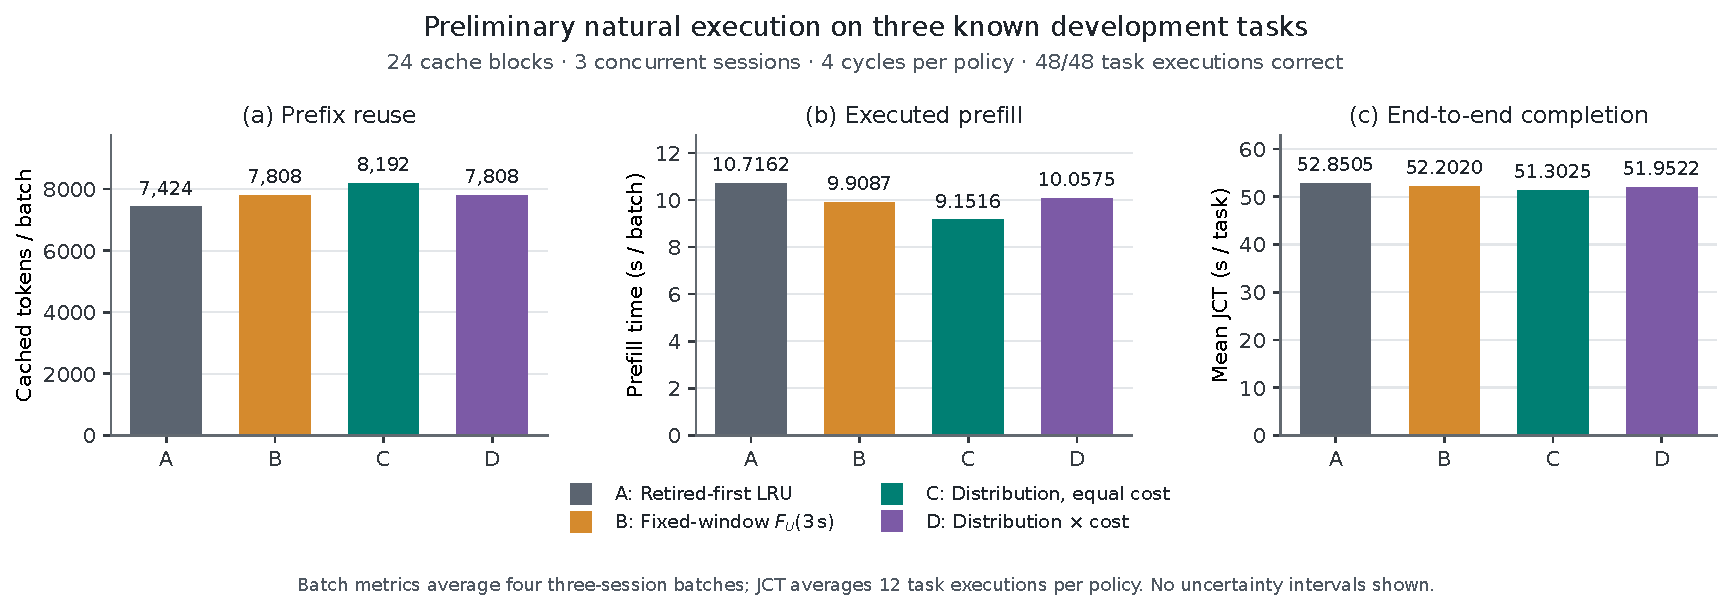
\includegraphics[width=\textwidth,keepaspectratio,alt={Completed preliminary comparison. Bars start at zero and show separate measurement levels: cached tokens and prefill seconds per three-session batch, and JCT seconds per task. Four repeated cycles per policy cover three known development tasks; no confidence intervals are inferred from these aggregates.}]{leasepath_isca_v2_assets/figures/figure2_preliminary_results.pdf}
\caption{Completed preliminary comparison. Bars start at zero and show
separate measurement levels: cached tokens and prefill seconds per
three-session batch, and JCT seconds per task. Four repeated cycles per
policy cover three known development tasks; no confidence intervals are
inferred from these aggregates.}\Description{The older three-task experiment compares cached tokens, prefill time and mean completion time across four policies.}
\label{fig:preliminary-results}
\end{figure*}

Both C--A and C--B mean-JCT differences are negative in all four cycles
(Figure 4). C--A ranges from \ensuremath{-}1.999 to \ensuremath{-}1.053 seconds; C--B ranges from
\ensuremath{-}1.621 to \ensuremath{-}0.423 seconds. The consistency is descriptive evidence within
these cycles, not a statistical generalization claim. Mean batch
makespan is 68.2116 seconds for A, 67.6207 for B, 66.4738 for C, and
67.1262 for D.

\begin{figure*}[t]
\centering
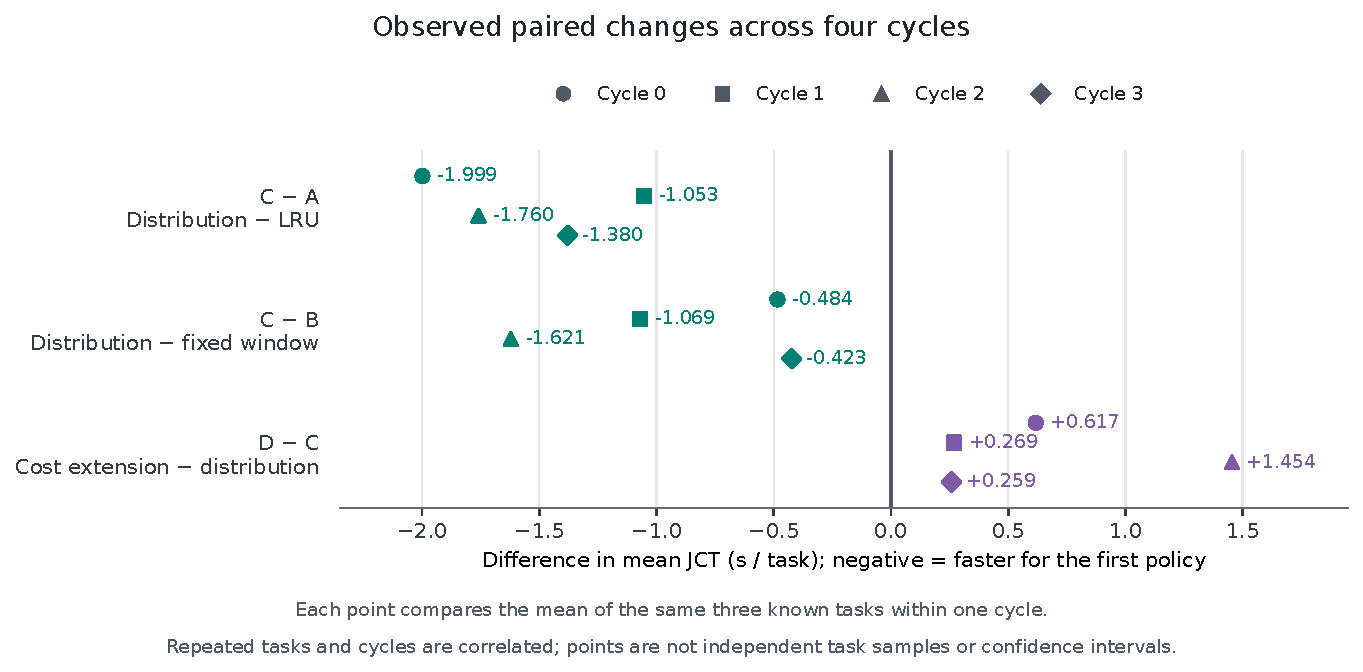
\includegraphics[width=\textwidth,keepaspectratio,alt={Within-cycle differences in mean JCT: negative C\ensuremath{-}A and C\ensuremath{-}B values favor equal-cost distribution scoring; positive D\ensuremath{-}C values favor equal cost over the cost extension. Each point is one repeated time cycle on the same three tasks, not an independent task-family sample.}]{leasepath_isca_v2_assets/figures/figure3_paired_cycles.pdf}
\caption{Within-cycle differences in mean JCT: negative C\ensuremath{-}A and C\ensuremath{-}B
values favor equal-cost distribution scoring; positive D\ensuremath{-}C values favor
equal cost over the cost extension. Each point is one repeated time
cycle on the same three tasks, not an independent task-family
sample.}\Description{Within-cycle completion-time differences for four repeated cycles of the same three development tasks.}
\label{fig:paired-cycles}
\end{figure*}

\subsection{A calibrated cost multiplier does not improve the
result}\label{a-calibrated-cost-multiplier-does-not-improve-the-result}

Adding marginal cost worsens mean JCT by 0.6497 seconds, or 1.266\%,
relative to equal-cost distribution scoring. D is slower than C in all
four cycles and reuses 384 fewer tokens per batch. This occurs despite
an independent 79-point calibration validation with mean absolute error
of 2.607 ms on its fixed prompt/length grid. There is no observed cost
or distribution fallback in these runs.

The request-level evidence helps identify the mismatch without resolving
its full cause. Relative to C, D loses 256 cached tokens on logistic
evaluation and 256 on temporal matching, while gaining 128 on ridge
validation. C and D have identical corresponding input and output
tokens. For one first-cycle logistic continuation, the actual request
has 1,777 tokens, while the previously observed block-aligned prefix has
1,536. C reuses 1,152 tokens and D reuses 896, with measured prefill of
0.87787 and 1.39069 seconds, respectively. The future 241-token
extension is used only in this post hoc diagnosis; it was not available
to the policy.

The cost table is calibrated on the observed prefix plus one token,
whereas later prompts include tool results and protocol text. Native
512-token batch boundaries and prefix dependencies can further change
the marginal value of a leaf. These are plausible explanations for the
proxy's failure, not independently isolated causal effects. The result
supports keeping equal cost as the current primary configuration, while
leaving the value of better causal cost models open.

\subsection{Completion-time attribution and controller
overhead}\label{completion-time-attribution-and-controller-overhead}

The natural experiment includes controller work, but it does not isolate
all causes of the observed JCT differences. Corresponding input tokens
are identical across policies. A and B average 651 generated tokens per
batch; C and D average 650. Thus comparisons between these groups
include a small output-length difference. Tool wall times also vary; for
example, mean logistic tool time is 9.3854 seconds under C and 10.5710
seconds under D. Even C--D, with matched input and output tokens, cannot
attribute its entire JCT difference to caching.

\begin{table*}[t]
\centering\small
\begin{tabular}{@{}
  >{\raggedright\arraybackslash}p{(\linewidth - 6\tabcolsep) * \real{0.2500}}
  >{\raggedleft\arraybackslash}p{(\linewidth - 6\tabcolsep) * \real{0.2500}}
  >{\raggedleft\arraybackslash}p{(\linewidth - 6\tabcolsep) * \real{0.2500}}
  >{\raggedleft\arraybackslash}p{(\linewidth - 6\tabcolsep) * \real{0.2500}}@{}}
\toprule\noalign{}
\begin{minipage}[b]{\linewidth}\raggedright
Policy
\end{minipage} & \begin{minipage}[b]{\linewidth}\raggedleft
Prediction ms / batch
\end{minipage} & \begin{minipage}[b]{\linewidth}\raggedleft
Logical admission + shadows ms / batch
\end{minipage} & \begin{minipage}[b]{\linewidth}\raggedleft
Controller prepare ms / batch
\end{minipage} \\
\midrule\noalign{}
\endhead
\bottomrule\noalign{}
\endlastfoot
A & 8.663 & 34.858 & 177.519 \\
B & 8.807 & 39.472 & 176.460 \\
C & 9.591 & 33.525 & 252.049 \\
D & 10.478 & 36.846 & 179.393 \\
\end{tabular}
\caption{Observed instrumentation categories, averaged over four three-session batches per policy. Categories overlap and must not be added. Controller preparation includes native inspection, deletion, and mapping work; it is not a direct timing of score integration alone.}
\end{table*}


LRU also incurs shadow-prediction auditing in this earlier experiment.
Therefore, the observed improvement over A is a net difference between
these instrumented configurations, not an established net gain over a
minimal LRU without shadow computation. Initialization and
page-residency preparation are outside the JCT window and have not been
amortized over workload size.

Physical and protocol audits support the validity of the measurement
chain: 157/157 requests map to the ledger, all 48 final answers
validate, and 96 real tool results are consumed by later requests. All
16 batches pass the specified zero-increment parent read-byte,
major-fault, and block-input gates. These checks cannot prove absence of
shared-host noise. Recorded CPU pressure spans 0.393\%--60.482\%, and
I/O pressure spans 1.094\%--5.777\%. The conclusions therefore remain
paired observations under this shared-server configuration.

\subsection{Continuous-agent reuse and end-to-end response}
\label{continuous-results}

\begin{table*}[t]
\centering\small
\caption{Continuous-agent development comparison: six projects, eight user turns each, six concurrent sessions, 150 persistent blocks. Every arm passes 48/48 turns with 244 model requests and 1,227,620 input tokens. Totals are per arm; response is averaged per user turn. This is one ordered cycle, without confidence intervals.}
\label{tab:continuous-e2e}
\setlength{\tabcolsep}{4pt}
\begin{tabular}{@{}lrrrrrrr@{}}
\toprule
Policy & Cached tokens & Prefill tokens & Prefill (s) & Saved & Response (s) & Saved & Updates \\
\midrule
Retired-first LRU & 433,536 & 794,084 & 1,602.567 & 0.00\% & 394.295 & 0.00\% & 0 \\
Empirical, dynamic, distribution & 718,464 & 509,156 & 981.421 & 38.76\% & 323.527 & 17.95\% & 2 \\
GBDT, static, distribution & 758,784 & 468,836 & 885.533 & 44.74\% & 316.997 & 19.60\% & 0 \\
GBDT, dynamic, fixed window & 761,984 & 465,636 & 889.837 & 44.47\% & 316.236 & 19.80\% & 2 \\
GBDT, dynamic, distribution & 762,880 & 464,740 & 883.732 & 44.86\% & 316.368 & 19.76\% & 2 \\
\bottomrule
\end{tabular}
\end{table*}


Table~\ref{tab:continuous-e2e} reports the new comparison separately
from the earlier three-task batches. All five arms execute the same
1,227,620 input tokens and validate 48/48 user turns. Dynamic GBDT
distribution scoring reuses 762,880 tokens versus LRU's 433,536:
329,344 additional cached tokens exactly replace the same amount of
executed prefill. Aggregate prefill time falls from 1,602.567 to
883.732 seconds, saving 718.835 seconds (44.86\%). Mean user-turn
response falls from 394.295 to 316.368 seconds, saving 77.927 seconds
(19.76\%). The other prediction policies reduce response by
17.95\%--19.80\%. This establishes an observed end-to-end difference
under real KV competition in these development histories, rather than
an offline prediction result alone.

\begin{figure*}[t]
\centering
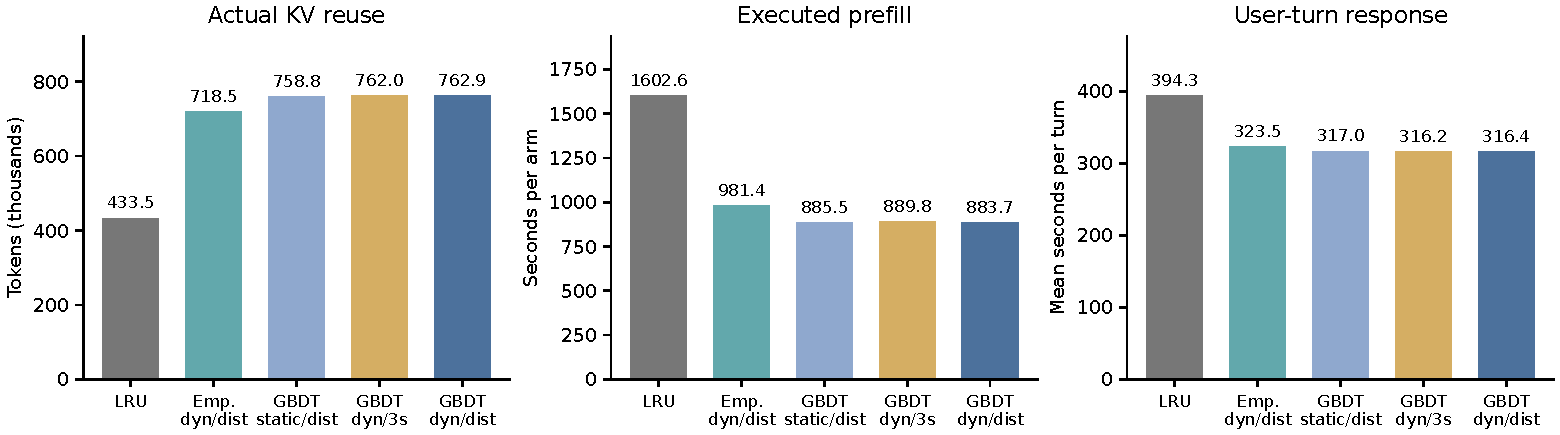
\includegraphics[width=\textwidth]{leasepath_isca_v2_assets/figures/figure5_continuous_e2e.pdf}
\caption{Continuous-agent development comparison. Each bar summarizes
one arm with 48 user turns across six authored projects. Axes start at
zero; aggregate prefill and average response have different units.
There are no repeated-cycle uncertainty estimates.}
\Description{Three bar charts show actual cached tokens, cumulative
prefill seconds, and mean user-turn response for the five policies. All
prediction arms improve these observed metrics over LRU; the three GBDT
arms are close.}
\label{fig:continuous-results}
\end{figure*}

The close GBDT results leave policy selection open. Dynamic distribution
reuses only 4,096 more tokens than static distribution and lowers mean
response by about 0.20\%. Relative to dynamic fixed-window scoring, it
reuses 896 more tokens but has about 0.04\% higher response. The
fixed-window arm is the cumulative probability \(F_U(3\,\mathrm{s})\),
not a prediction of a three-second return and not CacheWise. Neither
the extra value of online adaptation nor that of full distribution
scoring is established by these differences. A future empirical/GBDT
mixture requires its own causal training and ablation; it is not one of
the measured arms.

\subsection{Continuous-agent timing and prediction diagnostics}

\begin{table*}[t]
\centering\small
\caption{Measured timing categories for the continuous-agent comparison, in seconds per arm. Tools and background training overlap service; controller preparation includes prediction, so columns cannot be added to reconstruct a critical path. Model loading precedes the response window.}
\label{tab:continuous-overhead}
\setlength{\tabcolsep}{4pt}
\begin{tabular}{@{}lrrrrrrr@{}}
\toprule
Policy & Decode & Tools & Prediction & Preparation & Online fit & Load & Makespan \\
\midrule
Retired-first LRU & 1,796.477 & 20.510 & 0.000 & 25.342 & 0.000 & 30.180 & 3,641.511 \\
Empirical, dynamic, distribution & 1,797.064 & 20.688 & 0.299 & 26.618 & 0.742 & 34.336 & 3,039.848 \\
GBDT, static, distribution & 1,797.451 & 20.681 & 0.682 & 27.025 & 0.000 & 52.639 & 2,943.373 \\
GBDT, dynamic, fixed window & 1,797.536 & 20.198 & 0.740 & 27.750 & 0.983 & 88.545 & 2,955.819 \\
GBDT, dynamic, distribution & 1,797.737 & 20.583 & 0.758 & 27.758 & 1.041 & 178.907 & 2,950.107 \\
\bottomrule
\end{tabular}
\end{table*}


Decode totals span 1,796.477--1,797.737 seconds and actual tool execution
20.198--20.688 seconds across arms. The large measured change is in
prefill, with downstream queueing affecting response. This breakdown
supports the prefill mechanism but does not identify every second of
the response difference. Tools and training overlap service, and
controller preparation includes prediction. Summing these accumulated
categories would misrepresent a critical path. Model loading spans
30.180--178.907 seconds outside the steady-response window, indicating
that host conditions are not constant.

Dynamic distribution uses 0.758 seconds of aggregate prediction,
27.758 seconds of controller preparation, and 1.041 seconds of
background fit wall time (0.886 thread CPU seconds). Boundary data
preparation is also within measured response; fit time is not the whole
update overhead. Initial full-development fitting of both models takes
0.688 seconds, excluding the earlier diagnostic fits and model loading,
so it is not total startup cost. Empirical online updates are cheaper,
but the current cycle alone cannot determine a predictive policy's
long-run tradeoff between overhead and retained prefill savings.

\begin{table}[t]
\centering\small
\caption{Chronological diagnostic on 274 later snapshots of the same six development projects, after fitting on 805 earlier snapshots. Binary demand Brier, lower is better; not the three-class metric of Table 2 and not unseen-project evaluation.}
\label{tab:continuous-prediction}
\begin{tabular}{@{}rrr@{}}
\toprule
Horizon (s) & Empirical & GBDT \\
\midrule
1 & 0.00000 & 0.00278 \\
3 & 0.00103 & 0.00715 \\
10 & 0.08786 & 0.09980 \\
30 & 0.29652 & 0.27502 \\
\bottomrule
\end{tabular}
\end{table}


In the within-project chronological diagnostic
(Table~\ref{tab:continuous-prediction}), empirical prediction has lower
binary demand Brier at 1, 3, and 10 seconds, whereas GBDT is lower at
30 seconds. These are not directly comparable to the earlier
three-class scores: the data, features, weighting scale, split, and
metric differ. Better performance at one prediction horizon need not
yield better retention or response. Causal online prediction quality,
calibration, and drift response remain to be measured on independent
projects.

\subsection{Independent evaluation and policy selection remain open}

The six continuous projects exclude the old 50 parents, but were authored
and debugged during development. They do not establish source-independent
generalization. The six previously held-out source families remain
unused by these models; no independent main-result table is filled.
The older \(24/32/64\)-block pressure registration is a different
workload configuration, and its capacities cannot simply be reused for
these much longer untruncated requests.

The next controlled tests are balanced repeats, independent continuous
projects, a feasible capacity/concurrency matrix, and genuine changes
in tool duration and user return times. Predictor family, static versus
online training, and fixed-window versus distribution scoring need
separate contrasts, with a common frozen checkpoint for the scoring
contrast. Faithful CacheWise, TTL, and lifecycle-matched comparators
remain required for a complete-system claim. Predictor or hybrid choice
will use development evidence before a final test is unsealed.

\section{Limitations and Responsible Evaluation}
\label{limitations-and-responsible-evaluation}

The datasets are authored development workloads. The earlier 50-parent
collection has demand and retirement but no natural censoring; the new
continuous-agent snapshots all end in demand. Although retirement and
censoring are supported in the event interface, this does not validate
competing-risk prediction under cancellation, context replacement, or
long unresolved human waits. More snapshots from the same histories do
not supply independent projects or missing event types. Development
repairs and earlier failures must remain visible in any release.

The continuous projects add genuine iteration and causal queue state,
but tools are short and serial model service creates substantial
waiting. Their results need not predict behavior under long external
computations, broad branch structures, or a different arrival process.
Both the old coarse predictor and the new target-data predictor have
limited independent support. The scoring horizon, discount,
maximum-owner rule, and leaf-greedy eviction are engineering choices,
without a global JCT optimality guarantee.

System evidence covers one model, one native adapter, three GPUs split
by layers, 16K or 32K context, and serial FCFS model service. It does not
establish production continuous-batching behavior. The new five-arm
comparison has one fixed order on a shared server; model loading alone
shows host variation. It supplies observed reductions, not a population
significance claim. Its 48 correlated turns per arm are not 48
independent workloads. Static, dynamic, and fixed-window GBDT policies
are too close here to select a final policy, and no hybrid has been
validated. Balanced repeats, matched quality, independent projects,
stronger comparators, and startup/overhead amortization are still needed.

Tool permission and resource boundaries are part of the workload
contract. Released traces require review of sensitive inputs and
redistribution permissions. Reproducibility must preserve failed
attempts and distinguish constructed examples, chronological prediction
diagnostics, and natural execution. Public tool logs without actual
compatible backend lookup events are not ground-truth demand data.

\section{Conclusion}\label{conclusion}

LeasePath maps finite-horizon distributions of legal prefix demand to
feasible native KV retention actions. An initial fixed-predictor
experiment supports the equal-cost scoring configuration. A subsequent
six-project continuous-agent comparison shows 44.86\% less cumulative
prefill time and 19.76\% lower mean user-turn response for dynamic GBDT
distribution scoring than retired-first LRU, with identical per-owner
prompt sequences and accepted deliveries. Causal update audits show
that online fitting is deployable in the prototype. This development
cycle does not establish an advantage over static GBDT or fixed-window
probability scoring. Final predictor choice, possible mixtures,
independent generalization, and complete-system comparisons remain
open experimental questions.

\begin{acks}
The authors used generative AI tools to assist with language editing and to construct the workload schematic. The authors reviewed and take responsibility for all technical content, data, and claims.
\end{acks}

\section*{References}\label{references}
\small

Abhyankar, Reyna, Zijian He, Vikranth Srivatsa, Hao Zhang, and Yiying
Zhang. 2024. \emph{InferCept: Efficient Intercept Support for Augmented
Large Language Model Inference}. arXiv:2402.01869v2.
\href{https://arxiv.org/abs/2402.01869v2}{Specified version}.

Fu, Kaihua, Yukun Zhou, Chaokun Chang, Yinghao Yu, Luping Wang, Guodong Yang, Jiuchen Shi, Quan Chen, and Wei Wang.~2026. \emph{Capture the lifecycle: KV Cache
management in ReAct Agents with KVTether}. arXiv:2609.39819v1.
\href{https://arxiv.org/abs/2609.39819v1}{Specified version}.

Lee, Changhee, William R. Zame, Jinsung Yoon, and Mihaela van der
Schaar. 2018. \emph{DeepHit: A Deep Learning Approach to Survival
Analysis with Competing Risks}. AAAI.
\href{https://cdn.aaai.org/ojs/11842/11842-13-15370-1-2-20201228.pdf}{Official
paper}.

Li, Hanchen, Runyuan He, Qiuyang Mang, Qizheng Zhang, Huanzhi Mao, Xiaokun Chen, Hangrui Zhou, Huanchen Zhang, Alvin Cheung, Joseph Gonzalez, and Ion Stoica.~2025. \emph{Continuum: Efficient and Robust
Multi-Turn LLM Agent Scheduling with KV Cache Time-to-Live}.
arXiv:2511.02230. Version consulted: v7, September 8, 2026.
\href{https://arxiv.org/abs/2511.02230v7}{Specified version}.

Pan, Zaifeng, Ajjkumar Patel, Zhengding Hu, Yipeng Shen, Yue Guan, Wan-Lu Li, Lianhui Qin, Yida Wang, and Yufei Ding.~2025. \emph{KVFlow: Efficient Prefix Caching for
Accelerating LLM-Based Multi-Agent Workflows}. arXiv:2507.07400v1.
\href{https://arxiv.org/abs/2507.07400v1}{Specified version}.

Song, Zhenyu, Daniel S. Berger, Kai Li, and Wyatt Lloyd. 2020. \emph{Learning Relaxed Belady for
Content Distribution Network Caching}. In \emph{Proceedings of the 17th USENIX Symposium on Networked Systems Design and Implementation (NSDI 20)}, 529--544. USENIX Association.
\href{https://www.usenix.org/conference/nsdi20/presentation/song}{Publication page}.

Tiwari, Shubham, Tapan Chugh, Nash Rickert, Simon Peter, Ratul Mahajan,
and Haiying Shen. 2026. \emph{CacheWise: Understanding Workloads and
Optimizing KVCache Management for Efficiently Serving LLM Coding
Agents}. arXiv:2606.16824v1.
\href{https://arxiv.org/abs/2606.16824v1}{Specified version}.

Zheng, Haoyu, Fangcheng Fu, Jia Wu, Binhang Yuan, Yongqiang Zhang, Hao Wang, Yuanyuan Zhu, Xiao Yan, and Jiawei Jiang.~2026. \emph{Efficient Serving for Dynamic Agent
Workflows with Prediction-based KV-Cache Management}.
arXiv:2605.06472v1. \href{https://arxiv.org/abs/2605.06472v1}{Specified
version}.

\end{document}
